\chapter{Literature Review}%
\label{chapter:literatureReview}

\begin{introduction}
The chapter II covers a review of the literature about vehicle maintenance and service quality at the dealerships. 
Additionally, It analyses an existing system and compare with software solution of this dissertation.
\end{introduction} 


To acquire information about this topic I search information on the platform Scopus and Google Scholar. 
In Scopus, I used the query \"Vehicle AND Maintenance AND dealerships\" and found 49 papers.
On a primarly analysis from the title and abstract, I selected 24 papers that were related to this topic.
However, on a further examination, I chose to write about 3 papers in this dissertation. 
Most of the papers I discarded was because of the use of the words \"Vehicle\" and \"dealerships\". 
This words made the search return the papers that envisioned the dealerships as a reselling unit of the main company, which is not the focus of this dissertation.
Another reason was the use of machine learning to solve a specific problem, like predictive maintenance. 
While being a relevant approach, I decided to focus on Web Application and vehicle maintenace concepts.
In google scholar I found 3 papers about the electric vehicle in China. 
They may be important to understand the market in another country, however I chose to not include in this dissertation.  
The three papers I write in this dissertation were chosen because two of them were research studies about the process of vehicle maintenace and explain the importance of a quality of service in this industry.
The other paper described a solution implementation very similar to the use case of this dissertation.
With this three papers I could give a definition of the context and aquire some problems and solutions to focus on in the development fase.  



% \section{Background}

% The LightMobie is a company stablished in Águeda that provides a diverse set of products in the shared mobility sector. 
% The company also provides a software system to integrate with their bicycles and stations and vehicle maintenance.
% Currently, the company is in step of renewal of the system to a new solution of the bicycles and stations and is building a platform to interact and manage that system.
% This platform is able to visualize current and past information of the vehicle, stations and users and there interaction with each other.
% Additionally, alerts triggered by the equipment are also visible in the dashboard and the user can elaborate statistics on this data.


\section{Theoretical Concepts}

\subsection{Vehicle Maintenance}

Delivering vehicle maintenance services involves numerous activities, each crucial for maintaining service quality and ensuring customer satisfaction. 
Any deviation from these activities can negatively impact quality, leading to client dissatisfaction and loyalty lost. ~\cite{Setting_the_after_sale_process}
The loyalty of the client is the main source of income for the company, so it is important to maintain the quality of the service. ~\cite{Setting_the_after_sale_process}
To fufill this requirement at the fullest, one must supervise every stage of the process. ~\cite{Setting_the_after_sale_process}


\begin{figure}[h]
  \caption{Macro-level Flow of a vehicle maintenance or repair service. This figure was inspired by figure 6: After Sales process from ~\citet{Setting_the_after_sale_process}.}
  \centering
  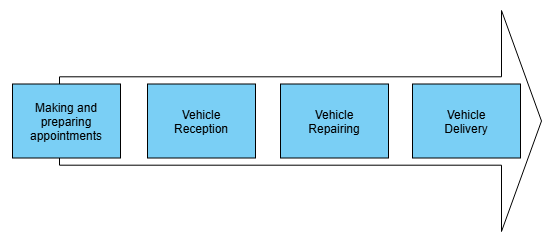
\includegraphics[width=0.50\textwidth]{figs/Vehicle_maintenace_macro}
  \label{fig:Vehicle_maintenace_macro}
\end{figure}

The general flow of a vehicle maintenance is illustrated in the figure \ref{fig:Vehicle_maintenace_macro}. 
The first step of the process starts with a client interacting with the garage to schedule a maintenance or repair. 
After that, the client goes to the garage, where the receptionist receives the client and the vehicle.
Here, the mechanic will perform the maintenance of the vehicle and, when is done, the vehicle will be delivered to the client.

To ensure quality in the first step the receptionist must understand the fill capacity of the garage and the time to complete the job. 
This step is very important because a mistake can lead to a break of promisses for the organization. ~\cite{Setting_the_after_sale_process}
The second step the receptionist and service advisor, when receiving the vehicle, must do a visual confirmation of the vehicle condition. ~\cite{Setting_the_after_sale_process}
In this step, the receptionist explains to the client the services of the garage and they both agreed with the services to be performed at a determined date. 
Then receptionist insert into the system this information. ~\cite{Setting_the_after_sale_process}

Following begins the third step and most important fase, the mechanic will perform the maintenance or repair on the vehicle. 
All of this process must be supervised by the quality control to ensure that the job is done correctly. ~\cite{Setting_the_after_sale_process}
This includes the repair process, extra work, final tests, vehicle wash, service report and date of delivery. ~\cite{Setting_the_after_sale_process}
To accomplish that the use of a checklist is recommended to ensure precision and accuracy at each step. ~\cite{Setting_the_after_sale_process}

Finally, the last step is the delivery of the vehicle to the client. 
In here, the admin must review the work done and the final price of the service to avoid extra payments from the client and incomplete payment to the workers. ~\cite{Setting_the_after_sale_process}

In this sense, the application of this dissertation will obey this flow.
For the receptionist and mechanic, the application will focus on reducing their mistake by giving accurate and illustrated information and turning the work more effective.
And for the administrator to control the quality of the service with assignment of tasks and authorization of purchases.  
Another user will be inserted into this flow, the warehouse operator, to manage the inventory of the dealership. 
The entire flow will be explained in chapter III. 

\subsection{Service Quality}
SERVQUAL is a service quality concept that provides a multidimensional approach for comparing consumers' perceptions of service quality against their expectations. 
It emphasizes five core dimensions ~\cite{SERVQUAL_OLD}:

\begin{itemize}
  \item Tangibles – Physical facilities, equipment, and appearance of personnel.
  \item Reliability – Ability to consistently deliver services as promised.
  \item Responsiveness – Willingness to assist the customer and proactivity.
  \item Assurance – Demonstrate courtesy and knowledge and inspire trust and confidence.
  \item Empathy – Caring and treat customers as individuals.
\end{itemize}

To measure the quality of the service one needs to do a questionnaire composed of 22 questions that are divided into the five dimensions of the SERVQUAL model. ~\cite{Measuring_After_sales_Service_Quality}
Each question must be divided into two answers, the first one is a score of the expectation of the service provided and the second one is score of the perception of the service received. ~\cite{Measuring_After_sales_Service_Quality}
The difference between the two answers is the quality of the service. ~\cite{servqual_blog_da_qualidade} ~\cite{Measuring_After_sales_Service_Quality} ~\cite{SERVQUAL_OLD}

% In some cases is recommended to do two interviews with the same client, one before the service to aquire the expectations and another after the service to aquire the perception. ~\cite{servqual_blog_da_qualidade}
In the paper ~\citet{Measuring_After_sales_Service_Quality} the authors used the SERVQUAL model to measure the quality of the service at a CMV SA dealership in South Africa.
The authors ~\citet{Measuring_After_sales_Service_Quality} collected the data from a semi-structured questionnaire and interviews with customers, managers, and staff.
The questionnaire was composed of 22 statements, that can be seen in the figure \ref{fig:SERVQUAL_results}, where the respondent used the Likert's point scale to rate the expectation and perception of each individual item.

The results seen in figure \ref{fig:SERVQUAL_results} revealed a negative score in all five dimensions. 
Even comparing the expectation of the customers with the expectation of the dealers the average score was negative (-0.10).
This shows that the services provided by the CMV SA dealer are not meeting the expectations of the customers and further improvements are needed. ~\cite{Measuring_After_sales_Service_Quality}
The customers recommendations included opening more workshops, to reduce travel inconvenience, and availability of parts, due to the long wait for the arrival from china.
The authors ~\citet{Measuring_After_sales_Service_Quality} emphasize the importance of the service quality the success of the business and recommend that the dealer should conduct regular SERVQUAL assessments to monitor and address service quality gaps. ~\cite{Measuring_After_sales_Service_Quality}

To address this issue, I will develop in this dissertation another application for the clients. 
This application will allow the users to evaluate the service done in this dealership, as well as some recommendations, following the model SERVQUAL. 

% \section{Increase Clients Satisfaction in Vehicle Maintenance}
% In belgrade, serbia, in 2013, a research was conducted to measure the satisfaction of the clients at dealerships. ~\cite{Setting_the_after_sale_process}
% In the reasearch, they divided the consumers' expectations or demands in three categories:
% \begin{itemize}
%   \item quality of repair work, service done within the agreed time schedule, price, friendliness and professionalism, the time waiting for an appointment. 
%   \item availability of spare parts, advice given for further maintenance, information given about additional work. 
%   \item adequate documentation about accomplished work, replacing vehicles, to invoices explained, café, Wi-Fi, phone availability. In this paper only the first category has been taken into consideration. 
% \end{itemize}



% The GAP model, precedent from the SERVQUAL, also measures service quality by identifying the difference between customer expectations and actual perceptions. 
% These gaps include discrepancies between customer expectations and management's understanding, management's perceptions and service specifications, service specifications and actual delivery, actual delivery and communicated services, and expected and delivered service. ~\cite{Measuring_After_sales_Service_Quality}

% https://forms.app/en/blog/gap-model-of-service

\section{Existing solution}


\section{Service Management for MAS Motors LLC}

MAS Motors LLC is a Toyota dealership that provides vehicle maintenance services in Libya.
This company handles the daily work manually using basic applications and paper documents.
This approach has proven to be ineffective with the expansion of the business and the company needs a more modern method. ~\cite{MAS_MOTORS}
So the author ~\citet{MAS_MOTORS} developed a web application that facilitates and increase the performance of the work at the dealership.

The system targets multiple user groups, such as service advisers, technicians, and customers, and offers a centralized platform to manage tasks like job card management, inventory updates, and customer service. ~\cite{MAS_MOTORS}
The authors' application was developed using the Laravel, which is a PHP web application framework, with MariaDB as the database management system, which is a popular open source relational database.

The authors ~\citet{MAS_MOTORS} applied \ac{RAD} methodology as a software development tool to develop the application, due to its feedback, flexibility and quickness.
\ac{RAD} is an agile software development approach that focuses on rapid prototyping and quick feedback from users over a costly planning. ~\cite{rapid_app_development}
This appreoach ideology is an ongoing testing and refinement of the project instead of following a detailed planning and design, such as traditional models.
It is composed of four phases: Define requirements, prototype, feedback, and final product. ~\cite{rapid_app_development}
The requirement phase is defined by the definition of an unrestricted set of requirements, that can be changed during any point in the cycle. 
In the prototype phase, the developers create a prototype of the system to Demonstrate to the client. 
This prototype may be rushed since in the finalization stage, the developers will refine the final product. ~\cite{rapid_app_development}
In the next phase, the feedback, developers present their work to the client and end-users.
Depending on the feedback, the client may want to change the requirements or add something new. In this case, the developers will go back to the second stage and repeat the process. ~\cite{rapid_app_development}
On a positive feedback, the client is satisfied by the prototype and the developers will move to the final product phase.
In this final phase, the developers will refine the prototype by optimizing their implementation. ~\cite{rapid_app_development}

For the first phase the authors write the requirements of the system following the Hewlett-Packard \ac{FURPS} model that categorize the software requirements into functional and non-functional aspects.
The acronym stands for:

\begin{itemize}
  \item Functionality – The core features and business-domain-specific aspects.
  \item Usability – User interface considerations like accessibility and aesthetics.
  \item Reliability – System availability, accuracy, and failure recovery.
  \item Performance – Metrics such as response time and throughput.
  \item Supportability – Testability, maintainability, and scalability.
\end{itemize}

The results of the application were positive, the survey response from employees and customers classified the system according to the \ac{FURPS} model with the scores 4.27 for functionality, 4.30 for usability, 4.27 for reliability, 4.46 for performance, and 3.36 for supportability.
Supportability was the lowest score, due to limited configuration options ~\cite{MAS_MOTORS}, however, the overall system improved the service efficiency and customer satisfaction. ~\cite{MAS_MOTORS}
The employees also recommended future enhancements, such as SMS notifications for service reminders, integrating social media, and expanding customer configuration options.

This SMS notifications functionality, will be planned in this dissertation Client application to inform the end of the maintenace and the availability for vehicle delivery.  


\section{Architecture Comparison}

% The architecture of the application will have a \ac{MVC} pattern. 
% The \ac{MVC} pattern separates the application into three main components: Model, View, and Controller.~\cite{mvc_geeksforgeeks} ~\cite{MVC_StartupHouse}
% The Model is responsable for the storage of data and the logic of the application.  ~\cite{mvc_geeksforgeeks} ~\cite{MVC_StartupHouse}
% It provides an abstraction layer of the database that allows data operation without the direct contact from the user interface. ~\cite{MVC_StartupHouse}
% The View represents the \ac{UI} of the application and is used to present the information from the Model component. ~\cite{mvc_geeksforgeeks} ~\cite{MVC_StartupHouse}
% This component is also responsable for the user's interactions and it does not contain any logic of the application, only limits itself to the communication between the Controller and the user. ~\cite{MVC_StartupHouse}
% The Controller is responsable to process the data and update the Model and the view, based on the user's actions. ~\cite{mvc_geeksforgeeks} ~\cite{MVC_StartupHouse}

% This pattern provides a clean separation of concerns, that increases the maintainability, reusability and testability of the code. ~\cite{mvc_geeksforgeeks} ~\cite{MVC_StartupHouse}
% This requirements are advantageous, since the natural agility of the requirements of the project are not fully stablished and may receive some suggestion from the company along the way. 
% The scalability is also important since the aim market of this application are the company's dealerships that may be scattered across the country or even Europe.

The framework the application will be built with is the Asp Net Core MVC. 
I believe this approach will be better than following the successful application from \citet{MAS_MOTORS} due to a variety of reasons shown in \ref{table:architetcture_comparison}.
Firstly, the integration with the microsoft framework MYSQL database is more simple when using ASP.NET Core due to the package Entity Framework. % [https://learn.microsoft.com/en-us/aspnet/entity-framework]
Laravel also supports this database interaction, but Asp Net Core MVC is more suitable for this environment. ~\cite{asp_net_vs_laravel}
Additionally, Laravel loses in performance with the Compiled Language ASP.NET since it is a Interpreted language. 
Finally, in security, laravel offers some security features like hashing or secure input validation, but requires deeper PHP knowledge and proactive vulnerability management. 
Microsoft offers greater security tools in ASP.NET Core mvc with role-based authentication and login management with Identity framework.
This functionalities provides a major abstraction to this concept and allows the develop to focus on the application functionalities. ~\cite{asp_net_vs_laravel}


\begin{table}[]
  \begin{tabular}{| m{5em} | m{15em} | m{15em} |}
    \hline
   Parameter & Laravel  & ASP.NET Core MVC   \\
   \hline
   Language & PHP &  C\#  \\
   \hline
   Performance &  Lower Performance due to being a Interpreted language & Higher performance due to being a Compiled language   \\
   \hline
   Security & Offers some Features like hashing and secure input validation &  Provides major abstraction with Microsoft tools   \\
   \hline
   Integration with SQL & Supports various relational databases & More recommended for Microsoft environments because of integration packages  \\
   \hline
  \end{tabular}
  \caption{Comparison of the Laravel and ASP.NET Core MVC frameworks on a web application development to be integrated in LightMobie Platform.}
  \label{table:architetcture_comparison}
  \end{table}

Another reason to use this framework is to integrate with the Fleet Management System that has the same approach. 
This way, despite turning the system more complex, some functionality like authentication and role assignment are already developed and only need integration. 
This integration is not a disadvantage since I was involved in the contruction of the system and I am familiar with the functionalities.






